\documentclass[12pt]{article}
\usepackage[english]{babel}
\usepackage{natbib}
\usepackage{url}
\usepackage[utf8x]{inputenc}
\usepackage{amsmath}
\usepackage{graphicx}
\graphicspath{{Images/}}
\usepackage{parskip}
\usepackage{fancyhdr}
\usepackage{vmargin}
\setmarginsrb{3 cm}{2.5 cm}{3 cm}{2.5 cm}{1 cm}{1.5 cm}{1 cm}{1.5 cm}

\title{Sondeos Meteorológicos de la atmósfera}								% Title
\author{Martha Anahí Iñiguez Beltrán}						% Author
\date{\today}											% Date

\makeatletter
\let\thetitle\@title
\let\theauthor\@author
\let\thedate\@date
\makeatother

\pagestyle{fancy}
\fancyhf{}
\rhead{Física Computacional}
\lhead{\thetitle}
\cfoot{\thepage}

\begin{document}

\begin{titlepage}
\centering
    \vspace*{0.5 cm}
    
\includegraphics[width=5cm]{unison.jpg}\\[1.0 cm]	% University Logo
    \textsc{\LARGE Universidad de Sonora}\\[2.0 cm]	% University Name
    \textsc{\Large Departamento de ciencias exactas}\\[1.0 cm]
\textsc{\Large Física Computacional}\\[0.5 cm]
\rule{\linewidth}{0.2 mm} \\[0.4 cm]
{ \huge \bfseries \thetitle}\\
\rule{\linewidth}{0.2 mm} \\[1.5 cm]
\begin{minipage}{0.6\textwidth}
\begin{flushleft} \large
\emph{Alumno:}\\
\theauthor
\end{flushleft}
\end{minipage}~
\begin{minipage}{0.4\textwidth}
\begin{flushright} \large
214202804
\end{flushright}
\end{minipage}\\[2 cm]


{\large \thedate}\\[2 cm]

\vfill

\end{titlepage}

\tableofcontents
\pagebreak

\section{Introducción}

En ésta actividad se analizaron los datos obtenidos por sondeos atmosfericos en la zona de Monterrey. Los datos fueron obtenidos del sitio de web de la Universidad de Wyoming, específicamente los datos de las fechas 22 de Diciembre y Junio del 2017.

En el desarrollo de ésta actividad retomaremos el uso de el lenguaje de programación Python, para el manejo de bases de datos utilizaremos la librería Pandas y para la interpretación de los datos nos apoyaremos con el graficador Matplotlib.

A continuación expondremos los fundamentos, análisis de datos y los resultados de ésta actividad.

\section{Fundamentos}

En princípio sabemos que la tierra tiene una capa de aire llamada atmósfera, éste es un gas compuesto de distintos elementos. La atmósfera tiene cinco capas principales: la exosfera, la troposfera, la estratosfera, la mesosfera y la termosfera. Cada capa tiene una composición y características distintas entre ellas lo que lleva a que los fenómenos físicos se lleven a cabo de distintas maneras. Los sondeos atmosféricos por globos instrumentados llevan a cabo la tarea de recolectar datos a distintas alturas de la atmosfera y compararlos entre sí para notar las características que varían entre las capas.

Los datos recopilados serán los que utilicemos para analizar y mostrar a través de gráficas las comparaciones anteriormente mencionadas.

\section{Análisis de datos} 

Para el análisis de datos tomaremos las dos bases de datos recopiladas con fechas del 22 de junio y 22 de diciembre del 2017. Después de exportarse las bibliotecas pandas y matplotlib comenzaremos leyendo los datos y saltando los primeros renglones, los cuales no tienen infromación útil. Utilizaremos la función "Data Frame" de pandas para dar estructura a los datos y posteriormente hacemos un análisis de los tipos de datos que manejaremos usando la función "describe".

Para finalizar, graficaremos los datos recopilados usando las funciones de de matplotlib. A continuación se muestra el código que utilizamos.

\begin{verbatim}
import pandas as pd
import numpy as np
import matplotlib.pyplot as plt

#procedemos a leer los datos de los archivos
junio=pd.read_csv('22JUN17.txt',skiprows=1,sep='\s+')

junio.head()

junio22=pd.DataFrame(junio)

junio22.dtypes

diciembre=pd.read_csv('22DIC17.txt', skiprows=1, sep='\s+')

diciembre22=pd.DataFrame(diciembre)

diciembre.head()

x=junio22.PRES

y=junio22.HGHT

plt.figure

plt.title('Presión contra altitud de Junio 22')

plt.plot(x,y)

plt.grid(True)

plt.xlabel('Presión')

plt.ylabel('altitud')

plt.show()


\end{verbatim}

\section{Resultados}

A continuación mostraremos las gráficas obtenidas a partir de los datos recopilados.


\begin{figure}
\begin{centering}
  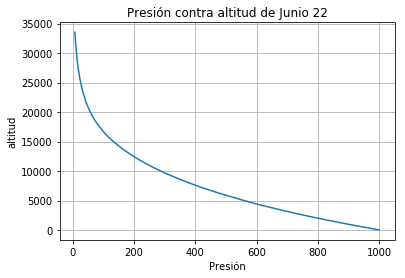
\includegraphics[scale = 0.8]{PRESALTJUN.png}
  \caption{Presión en función de la altura (junio 2017)}
\end{centering}
\end{figure}

\begin{figure}
\begin{centering}
  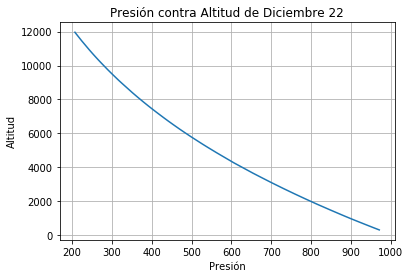
\includegraphics[scale = 0.8]{PRESALDIC.png}
  \caption{Presión en función de la altura (Diciembre 2017)}
\end{centering}
\end{figure}

\begin{figure}
\begin{centering}
  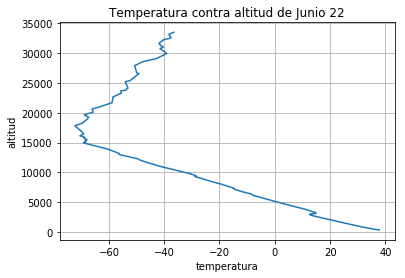
\includegraphics[scale = 0.8]{TEMPALTJUN.png}
  \caption{Temperatura en función de la altura}
\end{centering}
\end{figure}

\begin{figure}
\begin{centering}
  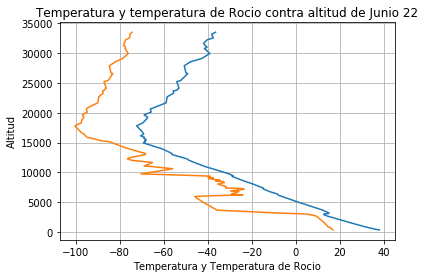
\includegraphics[scale = 0.8]{TEMPROCIOJUN.png}
  \caption{Temperatura de rocío en función de la altura (Junio 2017)}
\end{centering}
\end{figure}

\begin{figure}
\begin{centering}
  \includegraphics[scale = 0.8]{RAPVIEJUN.png}
  \caption{Rapidez de los vientos en función de la altura (Junio 2017)}
\end{centering}
\end{figure}

\begin{figure}
\begin{centering}
  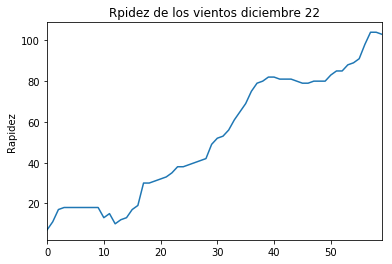
\includegraphics[scale = 0.8]{RAPVIEDIC.png}
  \caption{Rapidez de los vientos en función de la altura (Diciembre 2017)}
\end{centering}
\end{figure}

\begin{figure}
\begin{centering}
  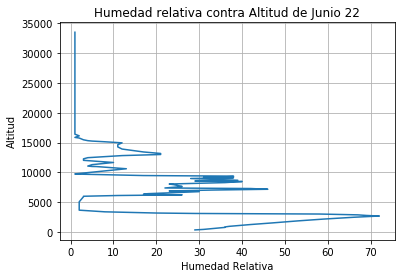
\includegraphics[scale = 0.8]{HUMRELJUN.png}
  \caption{Humedad relativa en función de la altura (Junio 2017)}
\end{centering}
\end{figure}

\begin{figure}
\begin{centering}
  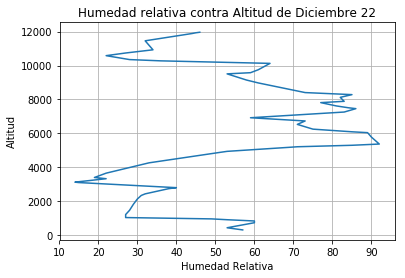
\includegraphics[scale = 0.8]{HUMRELDIC.png}
  \caption{Humedad relativa en función de la altura (Diciembre 2017)}
\end{centering}
\end{figure}


\section{Conclusión}

Por lo que muestran las gráficas podemos notar que los datos nos dicen que a mayor temperatura la presión baja y la temperatura aumenta, esto conocido anteriormente en el grupo de fluídos y fenómenos térmicos (Figura 1, 2 y 3).

La temperatura de rocío es la temperatura a la cual el aire debe descender para que el vapor de agua en el ambiente se condense. Ésta debe ser menor a la temperatura ambiental y conforme la altura aumenta la temperatura de rocío también debe descender al igual que la temperatura ambiental. En la gráfica de temperatura y temperatura de rocío se puede comprobar lo anterior mencionado (Figura 4).

En la gráfica de rapidez de los vientos podemos ver como ésta varía notablemente conforme mayor sea la altura, ésto probablemente a causa de las variaciones de temperatura en función de la altura (Figura 5 y 6).

Por último la gráfica de la humedad podemos notar como los datos en la tropopausia muestran que los niveles de la humedad se mantienen muy bajos o casi nulos. En las capas debajo de la anterior mencionada, existen muchas varíaciones en los niveles de humedad (Figura 7 y 8).

\section{Bibliografía}

- Atmosphere of Earth (2018) De wikipedia.org, Recuperado el 03 de marzo del 2018: $https://en.wikipedia.org/wiki/Atmosphere_of_Earth$

-Punto de Rocío (2018) De wikipedia.org. Recuperado el 03 de marzo del 2018: $https://es.wikipedia.org/wiki/Punto_de_rocio$

-Pandas: Powerfull Python data analysis toolkit (2018) De pandas.pydata.org. Recuperado el 03 de marzo del 2018: $https://pandas.pydata.org/pandas-docs/stable/index.html$

-Atmospheric Soundings (2018) College o Engineering, University of Wyoming. Recuperado el 03 de marzo del 2018: $http://weather.uwyo.edu/upperair/sounding.html$

\section{Apéndice}

A continuación se responderán unas preguntas acerca de la actividad.

\textbf{¿Cuál es tu opinión general de esta actividad?}

La actividad me pareció interesante ya que pudimos representar gráficamente fenómenos que conocíamos anteriormente. Aparte reforzamos el uso del lenguaje y las librerias.

\textbf{¿Qué fue lo que más te agradó? ¿Lo que menos te agradó?}

En general la actividad me gustó, no hubo nada en ella que no me gustara.

\textbf{¿Que consideras que aprendiste en esta actividad?}

Aprendí a graficar de manera más específica con matplotlib y tambíen como cambian las características de ciertos fenómenos físicos conforme a mayor altura se estudien.

\textbf{¿Qué le faltó? ¿O le sobró?}

La actividad estuvo completa e interesante.

\textbf{¿Que mejoras sugieres a la actividad?}

Ninguna. En mi opinión la actividad está bien elaborada para reforzar lo visto en la actividad 2.

\end{document}